\documentclass[12pt]{article}
\usepackage{fullpage}
\usepackage{amsmath, amssymb}
\usepackage{setspace}
\usepackage{graphicx}
\usepackage{enumerate}
\usepackage{times}
\usepackage{multirow}

\newcommand{\eps}{\epsilon}
\newcommand{\kap}{\kappa}
\newcommand{\lam}{\lambda}
\newcommand{\del}{\nabla}
\newcommand{\Msun}{\ensuremath{M_\odot}}

\renewcommand{\vec}[1]{\mathbf{#1}}
\newcommand{\mat}[1]{\mathbf{#1}}

\newcommand{\pp}[2]{\frac{\partial #1}{\partial #2}}

\title{Visualization of Angular Momentum Equilibration during Halo Mergers}
\author{Ryan Brewster \\ Peishi Jiang}

\begin{document}

\maketitle

\section{Introduction}

The energy and matter distribution in the modern universe displays a lot of
very complex structure. It is not well understood exactly how that distribution
evolved. The use of cosmological simulations can help shed light on the
formation of galaxies and other structures. In this context, large collections
of mass are called halos. The main goal of these simulations is to investigate
the formation of small halos and the process by which they merge together to
form the large, complex web of halos observed (or inferred) in the physical
universe.

The Dark Sky simulations  involve a large number of collisionless particles
interacting gravitationally. Though extensive optimizations are necessary due
to the scale of the simulations (over $10^{12}$ particles for the largest data
set), the underlying physical processes are very straightforward.

The computer program used to perform the Dark Sky simulations uses an adaptive
symplectic integrator to propagate the equations of motion for the system. It
also employs several approximations (none of which introduce significant
error), the most significant of which is a spatial tree data structure to make
it possible to approximate gravitational interaction between large collections
of particles.

The initial output of the simulation (henceforth called ``Level 1'' data) is
a series of timestep datasets, each of which contains the list of particle
positions and velocities at that timestep. Analysis of that data was performed,
yielding Level 2 data consisting of a list of halos for each timestep. These
halos were identified using the ROCKSTAR algorithm (which finds clusters of
particles in 6-dimensions space, 3 positional dimensions and 3 velocity
dimensions). ROCKSTAR itself stands for Robust Overdensity Calculation using
K-Space Topologically Adaptive Refinement. This algorithm has been extensively
optimized to provide both very accurate, robust identification of halos and
extremely high performance and parallelization capabilities. Finally, analysis
of the Level 2 data yielded Level 3 data consisting of a merger tree of halos
over time. This merger tree can help identify how halos form, merge together,
and separate over time.

Our goal for this visualization project is to find a way to display useful
information during the merging of several small halos into a larger halo. To do
this, we will specify a sequence of timesteps where several halos (at least
two) merge together to form a single halo; this should be possible using the
provided merger tree database. We will then identify all of the particles
involved in this process using the halo database. For each timestep in the
specified time step sequence, we will display every particle involved in the
halo merging. The particles will be colored by a function of their individual
properties (position, velocity) and their collective properties (angular
momentum, proximity from halo center, etc.).

We hypothesize that over the course of time, the distinct halos --- each of
which can be identified by the similar color of its constituent particles ---
will merge together and the particle colors will also quickly equilibrate to
form a homogeneous mix. If this is the case, it should be possible to identify
a time constant for this equilibration process. With the large number of halo
mergers that occur during the Dark Sky simulations, it may even be possible to
find a way to estimate the time constant from other parameters from the small
halos.


\section{Data Preprocessing}
In this contest, three types of data are provided for the halo identification
and analysis. The first is the raw particle data, which describes the state
(e.g., position of the particle, velocity of the particle, acceleration and so
forth).  The format of the file is SDF, including two parts (i.e., the layout
of the data (ASCII header) and the binary data). The second type of the data is
Hala catalog, describing the states of halos at each snapshot time, written in
plain text file.  And the final dataset type is Merger Tree database, including
the information of merger tree which ``links the individual halo catalogs that
each represents a snapshot in time''.

To identify the halos in each time step and investigate how the particles evolves to 
halos with time, it is crucial to conduct relevant numerical analysis on both raw 
particle datasets and information of halo and merger tree. Therefore, the unit conversion 
among the three data types is necessary. A short summary on the main elements in the 
raw particle datasets and halo catalog and merger tree is provided in Table 1.

\begin{table}[h]
\centering
\begin{tabular}{rll}
                          &  \textbf{Quantity} & \textbf{Unit} \\
\hline
\multirow{3}{*}{Particle\Huge\{} &  position          & kpc             \\
                                 &  velocity          & kpc/Gyr         \\
                                 &  mass              & $10^{10}$ \Msun \\
\hline
\multirow{3}{*}{Halo\Huge\{}     &  position          & Mpc/$h$ (comoving) \\
                                 &  velocity          & km/s (physical)  \\
                                 &  angular momentum  & $\Msun/h \cdot$ Mpc$/h \cdot$ km/s (physical)  \\
\end{tabular}
\caption {Units of main elements in the datasets}
\label{tab:units}
\end{table}

\section{Challenges}
\label{sec:challenges}
The provided dataset includes snapshots from the simulation run. These
snapshots are provided every 40 iterations or so. The greatest challenge that
we faced in this project was how to visualize an equilibration process which
takes place at a very fast timescale. Because the process takes place so
quickly (relative to the time between snapshots), we have very few datapoints
that are available during the process. We had initially hoped to be able to
actually animate the halo merger process and directly see the shifting
distribution of angular momenta as it equilibrated. However, the animations we
produced were unsatisfactory; the halos jump around a great deal between
snapshots, and we were unable to observe any gradual mixing.

\section{Data Analysis}
The objective of this visualization project is to simulate how two halos evolve with 
time and are combined with each other finally. Therefore, we need to tackle and present
the following issues: (1) identifying its belonging particles given a halo at each time 
step; (2) visualizing the magnitude of the angular momentum of each belonging particle 
in a specific halo; (3) animating the combination process of two halos over time;
(4) analyzing the change of particle angular momentum spectrum of two halos over time.

\subsection{Identifying a Halo's Constituent Particles}
The position information of particles (from the raw particle files
\verb@ds14_scivis_0128_e4_dt04_*@) and halos (from the halo list files
\verb@hlist_*@) at each time step are utilized to find the particles that make
up a given halo. Our process is as follows: first, choose a specific halo; this
can be done arbitrarily, or by identifying halos that have a desired property.
Next, we perform a coordinate transformation on the halo location, taking it
from the system used by the Rockstar algorithm to the system used by the
Darksky simulations (see Table \ref{tab:units} for the units used). This
transformation is a linear mapping of the form
\begin{equation}
f(\vec{r}) = \frac{10^3 a}{h} \vec{r} - \frac{L_0}{2}
\end{equation}
where $10^{3}$ converts from Mpc to kpc, $h$ is a parameter that encompasses
uncertainty in the Hubble constant, and $a$ is a scaling factor using by the
simulation. $L_0$ is the size of the simulation box. All of these parameters are
provided in the particle dataset headers.

The second step is to process the entire list of particles and filter out those
particles which are ``close'' to the halo location that we just computed.  We
use a simple radial cutoff as our metric for ``closeness''. The cutoff we chose
is the ratio of the virtual halo radius and the radius scale (both parameters
can be found in the Rockstar halo list). This step is extremely time-consuming,
because the number of particles is very large.  In principle there should be
a way to locate a halo's constituent particles more efficiently by using the
Morton-ordering of the particles themselves. Without this optimization, it is
difficult to apply our procedure to the largest data set.

Next, the angular momentum of each particle in its halo is computed using
its relative displacement from the halo center and its relative linear
momentum:
\begin{equation}
\vec{L} = (\vec{r_1} - \vec{r_h}) \times (\vec{p_1} - \vec{p_h})
\end{equation}
where $\vec{L}$ is the angular momentum of a particle; $\vec{r_1}$ and $\vec{r_h}$ are
the positions of the particle and the halo, respectively and $\vec{p_1}$ and $\vec{p_h}$ 
are the linear momentums of the particle and the halo, respectively.

Finally, VTK is used for the visualization of the particles of a specific halo
at each time step. To provide a general insight of how the particles move inside 
the halo (see Figure \ref{fig:halo_particles} for an example), we visualize the 
components of the particles' angular momentums parallel to the spinning angular 
momentum of their halo.
\begin{equation}
proj_{\vec{L_h}}(\vec{L}) = \frac{\vec{L} \cdot \vec{L_h}}{\abs{\vec{L_h}}}
\end{equation}
where $\vec{L_h}$ is the spinning angular momentum of a halo; $\vec{L} \cdot \vec{L_h}$
is the dot product of the angular momentums of all the particles and the mean 
angular momentum of their halo.

\begin{figure}[htp]
\centering
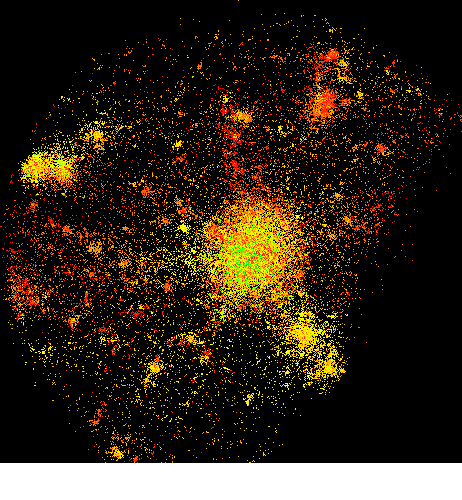
\includegraphics[width=0.5\columnwidth]{../figures/halo_particles.png}
\caption{A halo with its constituent particles colored by their angular momenta.}
\label{fig:halo_particles}
\end{figure}

\subsection{Simulating the movement of a halo's constituent particles}
Due to the big time lag between two adjacent time steps (around 40 iterations
or so) as described in Section 2, the animation of how the particles form a halo
is hard to be achieved based on the provided the raw particle datasets. Therefore, 
we simulate ''artificial'' raw particles (i.e., the position and the velocity of 
them) with a smaller time lag based on a given raw particles data sets through the
basic physical law, the gravitational law. VTK is used for animating the movement 
of a halo's constituent particles from the ''artificial'' raw particles.

\subsection{The combination process of two halos}
We expect to simulate how two halos, which are independent initially, are combined
into one halo finally. Such two halos are chosen as two the 'parent'' halos sharing 
the same ''child'' halo from the merger tree file \verb@hlist_*@. Then, for 
each halo, at every time step, the histogram of all its constituent particles' 
$proj_{\vec{L_h}}(\vec{L})$ is generated to see the distribution of the movement 
of the particles within the halo. Finally, the combination process of two halos can
be visualized through the evolving of the histogram of the two halos' $proj_{\vec{L_h}}(\vec{L})$
over time.

\section{Results}

\bibliography{writeup.bib}
\bibliographystyle{plain}

\end{document}
